\section{Implementation}
\label{sec:implementation}

\subsection{Proxy Re-encryption Library}
\label{sec:PRE}
%
We implemented a library for proxy re-encryption (PRE) in Go based on the AFGH proxy re-encryption scheme~\cite{05-ndss-improved_proxy_reencryption}.
In order to send a plaintext message, the sender first generates an AES key, then encrypts the message under that key.
Then, they encrypt that ciphertext and its AES key with the recipient's public key.
$$E(m) = E_{k^+}(k_{AES},E_{k_{AES}}(m))$$

Once received, the recipient can decrypt the message with their private key, then decrypt the ciphertext with the now-exposed AES key.

\color{red}TODO: make sure the encryption formula is correct,
and figure out the decryption formula to put here\color{black}
%

%
For proxy re-encryption, the ciphertext can be re-encrypted by a re-encryption key generated from the private key of the original recipient and the public key of the new recipient.
%
It is important to note that if the message is re-encrypted, a different decryption function must be used.
%
Both \texttt{Decrypt1} and \texttt{Decrypt2} are implemented in our PRE library, and there is a significant increase in latency for \texttt{Decrypt2}, which we'll discuss in \ref{sec:evaluation}


\subsection{\SystemName Library}
%
\SystemName defines a \texttt{SambaProxy} struct:

\begin{verbatim}
type SambaProxy struct {
	pp                *pre.PublicParams
	functionInstances map[FunctionId][]InstanceId
	instanceKeys      map[InstanceId]InstanceKeys
	functionLeaders   map[FunctionId]InstanceId
}
\end{verbatim}

The cloud provider plays the role of the \texttt{SambaProxy} in FaaS systems.
%
Individual function replicas, also called instances, can use the public parameters to generate their public-private keypair, and register their public key with the proxy.
%
The function instances map keeps track of what replicas belong to what function. Knative will be periodically polled to keep this updated.
%
The instance keys map keeps track of public keys and re-encryption keys for every instance known to \SystemName.
%
The proxy needs to maintain the function leaders map, since incoming requests will be encrypted to the leader instance of each function's set of replicas, so the proxy must request that re-encryption keys from the leader.
%
A multitude of methods are defined on this struct that handle instances' and clients' requests to set public keys, send messages, etc.


\SystemName also defines a \texttt{SambaInstance} struct representing an individual instance of a function:

\begin{verbatim}
type SambaInstance struct {
	Id           InstanceId
	KeyPair      *pre.KeyPair
	PublicParams *pre.PublicParams
}
\end{verbatim}

It contains an RSA key-pair, generated from the public parameters maintained by the proxy, which it also stores upon receiving them.
%
Like for the proxy, we've defined methods for instances to perform the tasks required of them such as handling (decrypting and acting on) messages, generating re-encryption keys when requested, etc.


%
\subsection{\SystemName-Lite System}
The \SystemName library exposes \texttt{En\-crypt}, \texttt{De\-crypt1}, \texttt{Decrypt\-2}, \texttt{Gen\-erate\-Re\-Encryption\-Key} and \texttt{ReEncrypt} methods.
\SystemName-Lite calls these methods to perform the necessary operations.
These methods perform some serialization and formatting tasks, as well as call similarly-named methods in the PRE library to perform the cryptographic tasks.
The \SystemName-Lite system itself contains four services that can be built and run to simulate the eventual fully-featured \SystemName system.

The \texttt{proxy} service boots a \texttt{SambaProxy} that runs an HTTP server exposing endpoints for registering keys, and sending messages. 
All messages coming into the system will be routed through the proxy, but encrypted to the leader instance of whatever function they're addressed to.
Since our PRE implementation doesn't require the proxy to learn the secret key of any function instance in order to re-encrypt, this system maintains confidentiality even in the case of an untrusted cloud provider, which would be running the proxy service.

The \texttt{alice} and \texttt{bob} services boot \texttt{SambaInstances} that request the public parameters from the proxy, generate public/private key-pairs for themselves, and register their public key back with the proxy. 
Then, they launch HTTP servers to which the proxy will make requests to send messages and request re-encryption keys.
We arbitrarily set \texttt{alice} to be the leader, which the sender encrypts to, and can toggle between her being able to handle requests and too busy to handle requests.
In the latter case, \texttt{proxy} requests a re-encryption key from \texttt{alice}, so that it can re-encrypt the message and send it to \texttt{bob}.
This re-encryption key between alice and bob only needs to be generated once per instance pair, the first time that a message must be re-encrypted from one instance to another.
This will be important to keep in mind when we explore the performance impact of the \SystemName operations in section~\ref{sec:evaluation}.

The \texttt{sender} service is a simple application that calls \texttt{samba\-.En\-crypt} to encrypt a message, and then decrypts the response.
Running these services in the specified order demonstrates the control flow of the \SystemName PRE system.

%% %
%% We will implement \SystemName within Oak and the
%% OpenFaaS~\footnote{\url{https://www.openfaas.com}} serverless platform.
%% %
%% For proxy re-encryption, we will explore integrating both bilinear
%% map~\cite{ 05-ndss-improved_proxy_reencryption} and post-quantum
%% lattice-based schemes~\cite{17-tops-fast_proxy_re_encryption}.
%% %
%% For aggregate signatures, we will use BLS
%% signatures~\cite{03-eurocrypt-aggregate_signatures_bilinear_maps,
%% 03-pkc-threshold_multi_blind_signatures}.


% [42] HelloRetail  Nordstrom. Hello, retail! https://github.com/ Nordstrom/hello-retail, 2018.
% [6] CodePipeline AWS. Aws-codepipeline-stepfunctions.  https://github.com/aws-samples/ aws-codepipeline-stepfunctions, 2018.
% [7] MapReduceAWS Lab. Lambda reference architecture for mapreduce. https://github.com/awslabs/ lambda-refarch-mapreduce, 2018.


%% \begin{figure}[t]
%%     \centering
%%     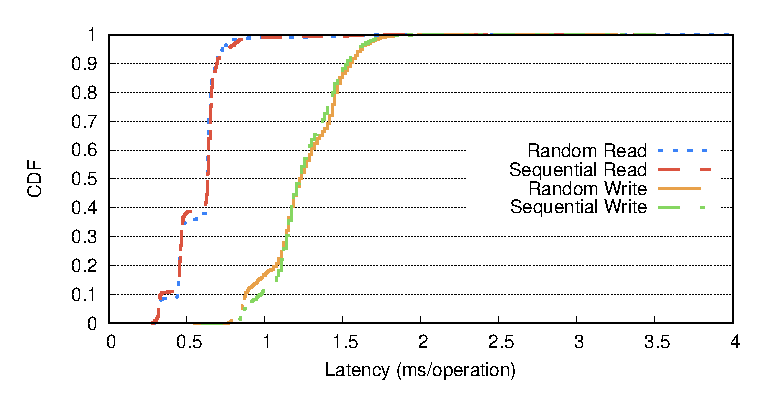
\includegraphics[width=0.5\textwidth]{figs/latency-cdf}
%%     %
%%     \caption{CDF of latencies for object read and write operations with \System (object size = 10M).}
%%     %
%%     \label{fig:latency-cdf}
%% \end{figure}
